\documentclass[usenames,dvipsnames,10pt]{beamer}
\usepackage[absolute,overlay]{textpos}

% Setup appearance:
\usetheme{Boadilla}
\usefonttheme[onlylarge]{structurebold}
\usecolortheme{seahorse}
\setbeamerfont*{frametitle}{size=\normalsize,series=\bfseries}
\setbeamertemplate{navigation symbols}{}
%\setbeamercolor{frametitle}{fg=Blue}
\renewcommand\alert[1]{{\color{Magenta} #1}}
\newcommand\program[1]{\texttt{#1}}

% Packages
\usepackage[english,ukrainian]{babel}
\usepackage{times}
\usepackage[T1]{fontenc}
\usepackage{color}
\usepackage{bm}
\usepackage{slashed}
\usepackage{booktabs}% http://ctan.org/pkg/booktabs
\usepackage{xspace}
\usepackage{multirow}
\usepackage{graphicx}
\newcommand{\tabitem}{~~\llap{\textbullet}~~}
\usepackage{minted}

\setlength{\fboxsep}{0pt}%
\setlength{\fboxrule}{1pt}%

%\definecolor{stcoupcolor}{RGB}{255,0,51}

% Setup TikZ
\usepackage{tikz}
\usetikzlibrary{arrows,shapes,backgrounds,positioning}
\tikzstyle{block}=[draw opacity=0.7,line width=1.4cm]

% arrows
\tikzset{
    myarrow/.style={
        draw,
        fill=orange,
        single arrow,
        rounded corners=1,
        %        width=2ex,
        minimum width=2ex,
        minimum height=3ex,
        single arrow head extend=1ex
    }
}
\newcommand{\arrowup}{\tikz [baseline=-0.5ex]{\node [myarrow,rotate=90] {};}}
\newcommand{\arrowdown}{\tikz [baseline=-0.5ex]{\node [myarrow,rotate=-90] {};}}
\newcommand{\arrowright}{\tikz [baseline=-0.5ex]{\node [myarrow,rotate=0] {};}}
\newcommand{\arrowleft}{\tikz [baseline=-0.5ex]{\node [myarrow,rotate=180] {};}}

% draw connection
\newcommand{\tikzmark}[1]{\tikz[remember picture] \node[coordinate] (#1) {#1};}

% page numbering (backup)
\newcommand{\backupbegin}{\newcounter{finalframe}\setcounter{finalframe}{\value{framenumber}}}
\newcommand{\backupend}{\setcounter{framenumber}{\value{finalframe}}}

% Author, Title, etc.
\title[Title]{\large Title}
\author[Олександр Зенаєв]{Олександр Зенаєв}
\date{}

% block with custom width
\newenvironment<>{varblock}[2][.9\textwidth]{%
    \setlength{\textwidth}{#1}
    \begin{actionenv}#3%
        \def\insertblocktitle{#2}%
        \par%
        \usebeamertemplate{block begin}}
    {\par%
        \usebeamertemplate{block end}%
\end{actionenv}}

\setbeamertemplate{itemize/enumerate body begin}{\footnotesize}
\setbeamertemplate{itemize/enumerate subbody begin}{\footnotesize}

\tikzset{
    every overlay node/.style={
        rounded corners,anchor=north west,
    },
}
\def\tikzoverlay{%
    \tikz[baseline,overlay]\node[every overlay node]
}%

% main part
\begin{document}
    \begin{frame}[plain]
    %\centering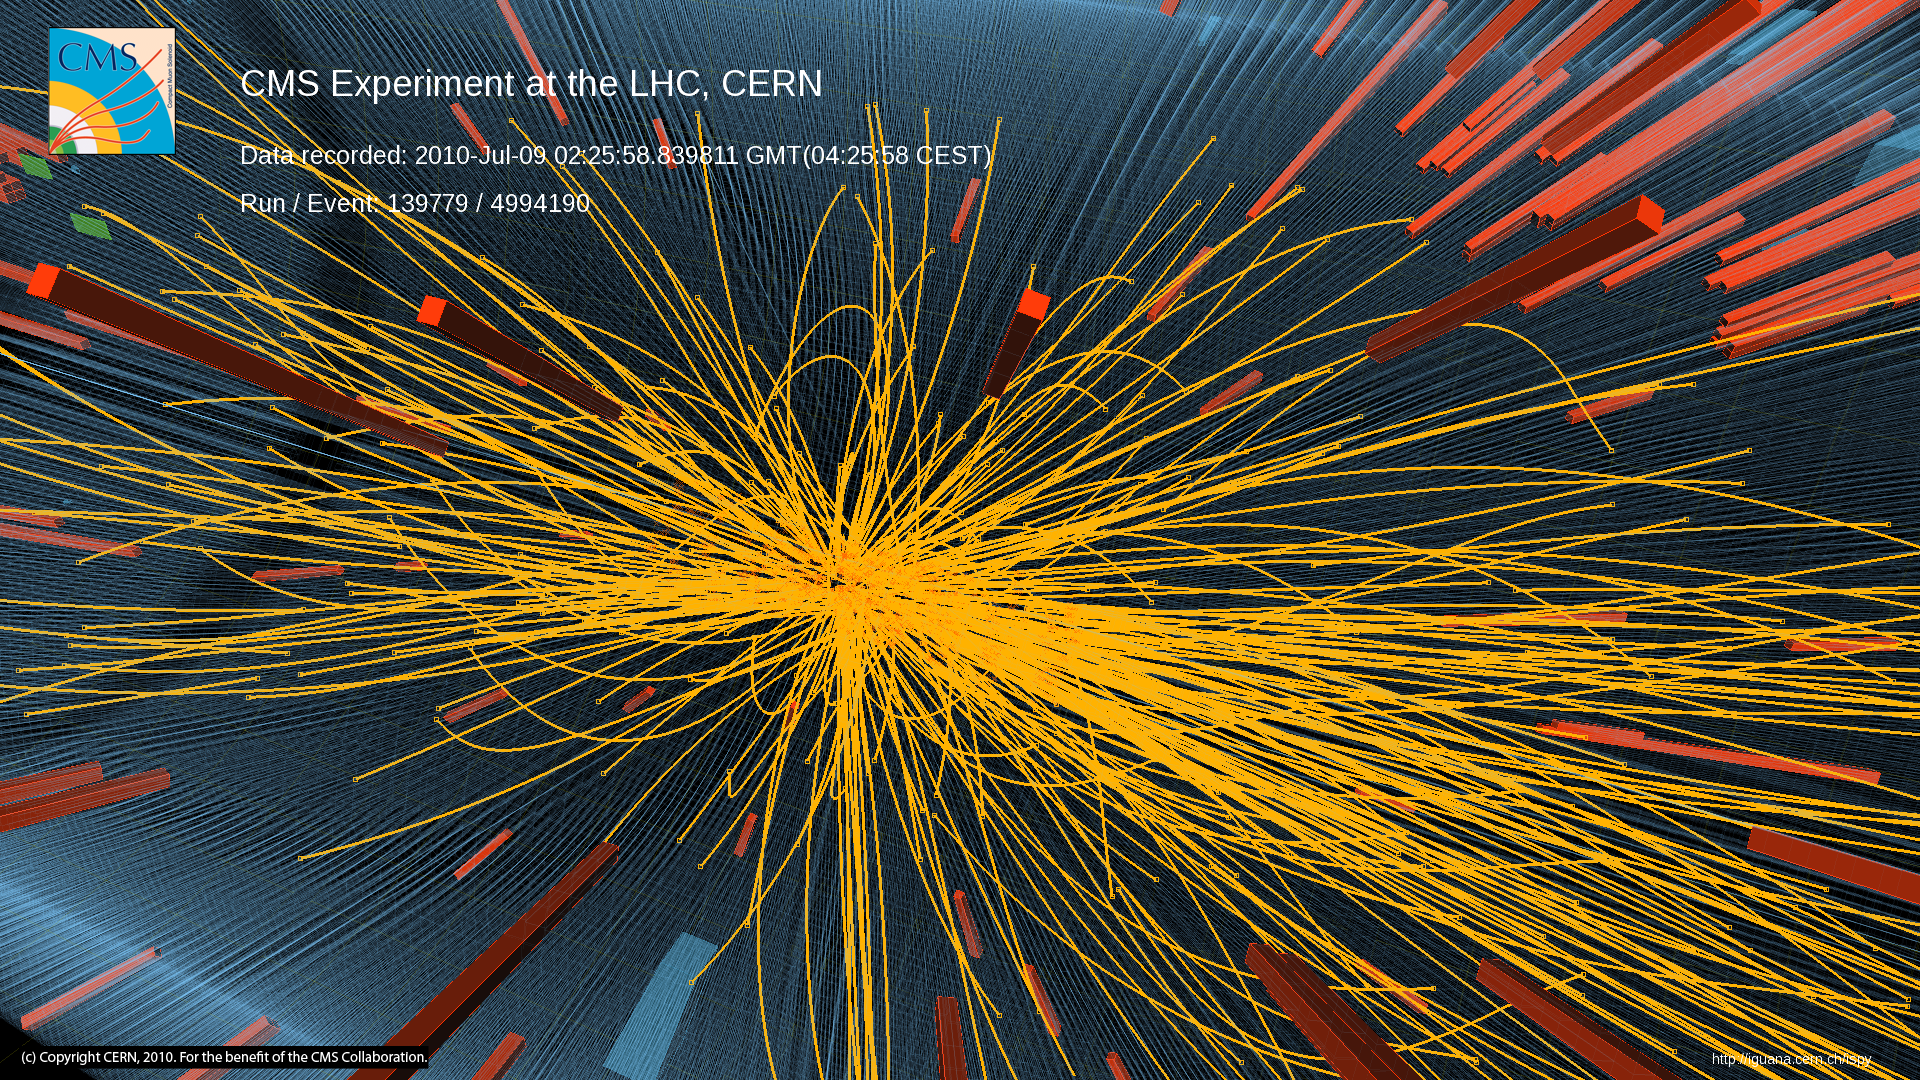
\includegraphics[width=0.15\textwidth]{pics/logo/cms.png}
    %\hspace{0.1\textwidth}
    %\centering\includegraphics[width=0.18\textwidth]{pics/logo/h1}
    %\hspace{0.1\textwidth}
    %\centering\includegraphics[width=0.15\textwidth]{pics/logo/desyNEW}
    %\hspace{0.1\textwidth}
    %\centering\includegraphics[width=0.15\textwidth]{pics/logo/zeus}
    %\hspace{0.1\textwidth}
    %\centering\includegraphics[width=0.15\textwidth]{pics/logo/xFitterLogo1.png}
    
    \vspace{-0.05\textheight}
    \titlepage
    
    %\vspace{-0.15\textheight}
    %\centering\includegraphics[width=0.4\textwidth]{pics/titlepic.jpg}

    %\vspace{-0.15\textheight}
    %{\color{blue} Overview:}
    
    \vspace{0.04\textheight}
    \centering
    %place \\
    %date
\end{frame}

% number of slides w/out backup
\renewcommand{\inserttotalframenumber}{2}
\setbeamercolor{footline}{fg=blue}
\setbeamerfont{footline}{series=\bfseries}


%\begin{frame}
%\frametitle{Status of xFitter releases}
%\begin{columns}\column{\dimexpr\paperwidth-10pt}
%\centering{\includegraphics[width=1.0\textwidth]{pics/pic.png}}
%\end{columns}
%\end{frame}

%\appendix
%\backupbegin
%\begin{frame}
%\frametitle{}
%\centering{\Huge \bf BACKUP}
%\end{frame}
%\backupend

\end{document}
